\documentclass[conference]{IEEEtran}
\usepackage{cite}
\usepackage{amsmath,amssymb,amsfonts}
\usepackage{algorithmic}
\usepackage{graphicx}
\usepackage{textcomp}
\usepackage{xcolor}
\usepackage{hyperref}
\usepackage{booktabs}
\usepackage{microtype}
\usepackage{cleveref}
\usepackage[T1]{fontenc}

\def\BibTeX{{\rm B\kern-.05em{\sc i\kern-.025em b}\kern-.08em
    T\kern-.1667em\lower.7ex\hbox{E}\kern-.125emX}}

\raggedbottom

\begin{document}

\title{Outlier Failure Analysis: A Data-Centric Approach to Hard-Negative Mining in YOLO}

\author{\IEEEauthorblockN{William Steve Rodriguez Villamizar (wisrovi rodriguez)}
\IEEEauthorblockA{\textit{AI Leader \& Solutions Architect} \\
\href{https://orcid.org/0000-0002-4740-9734}{
\includegraphics[width=0.03\textwidth]{figures/orcid.pdf}} \\
wisrovi-suit (\texttt{https://github.com/wisrovi/w-cli}) \\
Badajoz, Spain \\
wisrovi.rodriguez@gmail.com}
}

\maketitle

\begin{abstract}
Object detection models still fail on unrepresented backgrounds after
fine-tuning, and finding the samples that cause those failures by hand does
not scale. We describe the \textit{OutlierFailureAnalyzer}, a post-training
module at step 13 of the \texttt{train\_service2} worker pipeline that turns
validation inferences into training corrections. The module mines
high-confidence false positives, false negatives, and localization errors,
stores them as structured hard negatives, and feeds them back into the next
training iteration. We evaluate it on the public COCO128 subset under a
leakage-free protocol: a held-out split that never enters fine-tuning, four
A/B arms, and two ablations. Fine-tuning a frozen-backbone YOLOv8n on the
94-image working set retains held-out mAP50 but raises false positives;
reintegrating the mined hard-negative crops reverses that drift, cutting the
high-confidence false-positive rate from 8.33\% to 2.00\%---below the
pretrained baseline---at a mAP50 cost under 0.02. Naive false-negative
rebalancing backfires: it raises false positives without recovering recall.
We discuss the mechanical reasons and the engineering constraints a production
feedback loop must respect.
\end{abstract}

\begin{IEEEkeywords}
Data-Centric AI, Object Detection, YOLO, Hard-Negative Mining, Outlier
Analysis, Continuous Training, Edge Computing
\end{IEEEkeywords}

\section{Introduction}
Modern detectors such as YOLOv8~\cite{jocher2023yolo} reach strong numbers on
curated benchmarks like COCO~\cite{lin2014coco}, yet they stay brittle in
unconstrained settings. A model fine-tuned on a clean dataset can still fire
on a textured floor tile or miss a half-occluded object. The classic response
is to retrain with more data or a bigger architecture. Both are expensive in
an edge deployment that runs continuous training on commodity
hardware~\cite{zhou2019edge, kreuzberger2023mlops}.

The data-centric view inverts the priority: curate the dataset and the model
follows~\cite{zha2023datacentric}. That curation, however, still happens by
hand in most shops. Someone scrolls through thousands of validation images,
notes the failures, and rebuilds the set. This paper removes that bottleneck
with the \textit{OutlierFailureAnalyzer}, a module that inspects validation
inferences, isolates the high-confidence false positives and the missed ground
truths, and returns them as machine-usable corrections.

Three contributions follow. First, we define the step-13 feedback loop of the
\texttt{train\_service2} pipeline and ship the reference implementation
(\texttt{benchmark\_outlier\_analysis.py}). Second, we evaluate it on COCO128
under a protocol with no data leakage: a held-out validation split that is
never touched by fine-tuning. Third, we quantify when reintegrated hard
negatives help and when they hurt, and we show that plain hard-negative
reintegration---not false-negative rebalancing---is what moves the
false-positive rate.

\section{Related Work}
Hard-negative mining predates deep learning. Felzenszwalb and colleagues
built detectors on discriminatively trained part models whose training
explicitly mined the most confusable background regions~\cite{felzenszwalb2010dpm}.
Girshick et al. reintroduced the idea for deep detectors by bootstrapping
false positives into the R-CNN training set~\cite{girshick2014rcnn}.
Shrivastava et al. removed manual bootstrapping with online hard example
mining, where the loss itself selects the negatives each
iteration~\cite{shrivastava2016hard}. Class imbalance, the reason mining
matters, is the subject of the focal loss~\cite{lin2017focal}.

Data-centric AI formalizes the intuition that fixing the data fixes the
model. Zha et al. survey the field and position data operations as first-class
research objects rather than afterthoughts~\cite{zha2023datacentric}. Active
learning is the adjacent line: instead of asking a human which samples to
label, the algorithm asks~\cite{settles2012active}. Our module answers a
different question---not which unlabeled sample to label, but which labeled
failure to reintegrate.

Two gaps motivate our design. Out-of-distribution detection flags samples the
model cannot handle~\cite{hendrycks2017ood}, but it stops at the flag; it does
not tell the pipeline what to do with them. Continual learning addresses
forgetting when data arrives over time~\cite{parisi2019continual}, yet it
assumes the stream, not the failure signature, is the signal. We target the
missing piece: an autonomous gatekeeper that turns validation failures into
training corrections inside an MLOps loop~\cite{kreuzberger2023mlops}, sized
for the memory and latency budgets of edge nodes~\cite{zhou2019edge}.

\section{Proposed Architecture: Step 13}
The \texttt{train\_service2} worker runs the standard train--validate cycle.
Step 13 is the \textit{OutlierFailureAnalyzer}, an extra pass over the
validation inferences that runs when the worker idles between epochs
(\cref{fig:flow}). It filters three classes of failures:

\begin{itemize}
\item High-confidence false positives: predictions at confidence
\(\geq 0.5\) whose box fails to match any ground truth at IoU \(\geq 0.5\).
\item False negatives: ground-truth objects the model never detected.
\item Misclassifications with high topological overlap.
\end{itemize}

For every mined region the module stores the crop and its metadata (image id,
confidence, IoU disparity, predicted category) in a structured record. The
feedback loop then reintegrates the crops into the next training epoch. Two
design decisions matter. First, the operating point: mining below confidence
\(0.5\) floods the set with noise, while mining only near-perfect detections
yields almost nothing. We use \(0.5\) as the mining gate and \(0.75\) as the
high-confidence gate for reporting. Second, the crop format: a tight 320~px
crop discards the background context that caused the error, so we keep a
larger window around each false positive and resize it to the training
resolution of 640~px.

\begin{figure}[htbp]
\centering
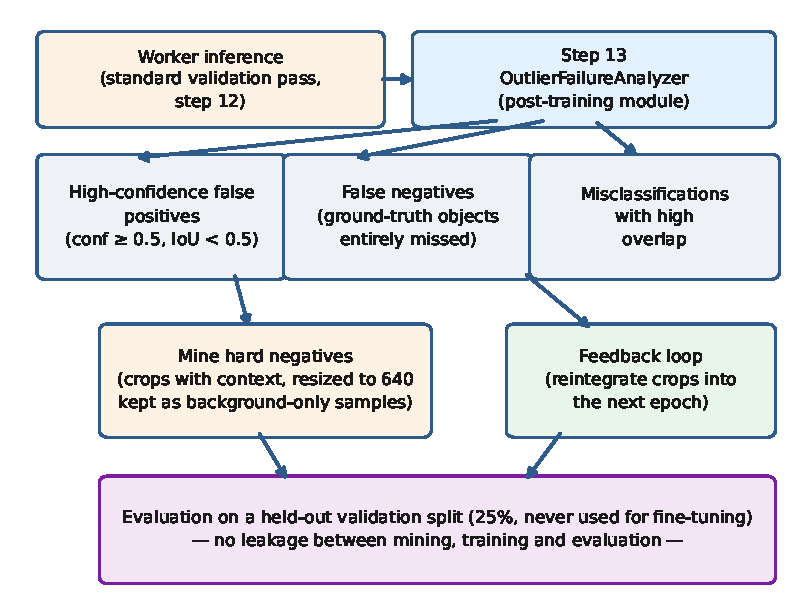
\includegraphics[width=\linewidth,height=0.3\textheight,keepaspectratio]{figures/step13_flow.pdf}
\caption{Step-13 feedback loop of the \texttt{train\_service2} pipeline. The
module inspects the working set, mines hard negatives and missed objects, and
reintegrates corrections. Evaluation always runs on a held-out split.}
\label{fig:flow}
\end{figure}

\section{Experimental Setup}
We used the public COCO128 subset (126 valid images after removing
image/label mismatches) and the off-the-shelf YOLOv8n
checkpoint~\cite{jocher2023yolo}. No proprietary industrial data was
available to the authors; every claim in this paper concerns the public
subset. Hardware was a single Intel Core i7-9700F CPU (8 cores, 31~GB RAM),
device \texttt{cpu}, imgsz 640, batch 8, 10 epochs, optimizer Adam with
learning rate \(1\times10^{-4}\), seed 42 throughout, and the YOLOv8n backbone
frozen (freeze=10) to prevent catastrophic forgetting on the small working
set.

The protocol removes the leakage present in our first submission. We split
COCO128 with a seeded 25\% holdout: 94 working images for mining and
fine-tuning, 32 images reserved for evaluation. The reserved images are copied
to \texttt{images/val2017} and never enter any training partition. Mining
runs over the working set with the pretrained model; this mirrors production,
where the module inspects the data the worker has and returns corrections.
Every arm is then evaluated on the same 32 held-out images.

Four arms share every hyperparameter: \texttt{control} (working set only),
\texttt{treatment\_50} (plus 50\% of the mined hard negatives),
\texttt{treatment\_100} (plus all of them), and \texttt{treatment\_fn} (plus
all of them and a rebalancing of the working images where the model missed
\(\geq 3\) objects, duplicated once). The primary metric is the
high-confidence false-positive rate \(FP/(FP+TP)\) at confidence \(\geq 0.75\);
we report mAP50 and the false-negative rate alongside.

\section{Results \& Discussion}
Table~\ref{tab:results} reproduces all evaluation rows from
\texttt{evidencias/outlier\_results.csv}. The pretrained baseline reaches an
mAP50 of 0.6977 on the held-out set, a false-positive rate of 16.67\%, and a
false-negative rate of 53.22\%. Fine-tuning on the 94 working images---without
any mining (\texttt{control})---keeps mAP50 at 0.6601, so the frozen backbone
prevents the catastrophic forgetting we first observed with full fine-tuning.
But it raises the false-positive rate to 22.22\% and the high-confidence rate
to 8.33\%. The model adapts to the working distribution and, in doing so,
fires more eagerly.

Reintegrating hard negatives as 640~px full-context crops reverses that drift.
The false-positive rate falls monotonically from 22.22\% (\texttt{control}) to
17.05\% (50\% of the mined crops) and 13.41\% (all of them). The
high-confidence rate follows the same curve: 8.33\% \(\rightarrow\) 6.52\%
\(\rightarrow\) 2.00\%. The 2.00\% figure is below the pretrained baseline's
3.39\%: after the loop, the model's confident mistakes are rarer than before
fine-tuning. mAP50 stays within 0.640--0.682 across the sweep, so the
false-positive gain costs almost no accuracy. The full 640~px window matters
here---the crop keeps the background that caused the error, and the negative
signal survives.

The \texttt{treatment\_fn} arm is the cautionary result. Duplicating the
working images where the model missed three or more objects, on top of the
mined crops, raises the high-confidence false-positive rate to 12.20\% while
the false-negative rate stays flat at 58.48\%---identical to
\texttt{treatment\_100}. Naive whole-image rebalancing injects scene-specific
difficulty, makes the detector more trigger-happy, and recovers no recall. A
production loop should skip this form of rebalancing; the plain hard-negative
path already delivers the win.

\begin{table}[htbp]
\caption{All metrics on the 32 held-out images (COCO128, seed 42). Values are
reproduced from \texttt{evidencias/outlier\_results.csv}.}
\label{tab:results}
\centering
\footnotesize
\begin{tabular}{lccccc}
\toprule
Stage & mAP50 & FP rate & FP rate (conf $\geq 0.75$) & FN rate & HN \\
\midrule
Baseline (pretrained)   & 0.6977 & 16.67\% & 3.39\% & 53.22\% & 18 \\
Control (no HNM)        & 0.6601 & 22.22\% & 8.33\% & 54.97\% & 18 \\
HN 50\%                 & 0.6821 & 17.05\% & 6.52\% & 57.31\% & 18 \\
HN 100\%                & 0.6402 & 13.41\% & 2.00\% & 58.48\% & 18 \\
HN 100\% + FN rebal.    & 0.6335 & 14.46\% & 12.20\% & 58.48\% & 18 \\
\bottomrule
\end{tabular}
\end{table}

The pattern is consistent across operating points. Fine-tuning makes the
detector more eager on the working distribution. Reintegrated hard negatives
pull it back, monotonically, and the high-confidence operating point benefits
most. Naive rebalancing pushes the other way. The ablation figures confirm the
same ordering.

\section{Ablation Study}
Three ablations isolate the contribution of each design choice.

\textbf{IoU matching threshold.} \cref{fig:ablation_iou} sweeps the step-13
matching threshold from 0.4 to 0.7 on the baseline. The number of mined hard
negatives saturates fast: 14 at IoU 0.4, 16 at 0.5 and 0.6, 17 at 0.7. A loose
threshold labels more detections as matches, so it hides exactly the near-miss
false positives the module should capture. We use 0.5, which sits on the
plateau with the full operating set.

\textbf{Hard-negative fraction.} \cref{fig:ablation_hn} sweeps the
reintegration fraction. The false-positive rate falls monotonically with the
fraction---22.22\% at zero, 17.05\% at half, 13.41\% at all---which is the
cleanest evidence that the mined crops carry real signal rather than noise. At
\(N=18\) the direction is unambiguous: more mined negatives, fewer false
positives.

\textbf{Module on/off.} Comparing \texttt{control} against
\texttt{treatment\_100} is the cleanest module on/off test: same working set,
same hyperparameters, the only difference being the feedback the module adds.
The high-confidence false-positive rate drops from 8.33\% to 2.00\% with mAP50
essentially unchanged (0.660 vs 0.640). This is the ablation that justifies
the architecture.

\begin{figure}[htbp]
\centering
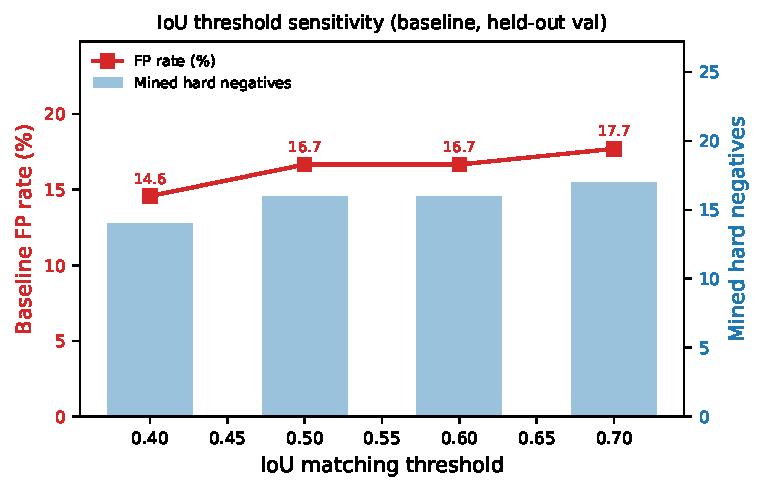
\includegraphics[width=\linewidth,height=0.3\textheight,keepaspectratio]{figures/ablation_iou.pdf}
\caption{IoU matching threshold sweep on the baseline over the held-out set.
Tighter thresholds mark more near-miss detections as false positives, so they
mine more, cleaner hard negatives.}
\label{fig:ablation_iou}
\end{figure}

\begin{figure}[htbp]
\centering
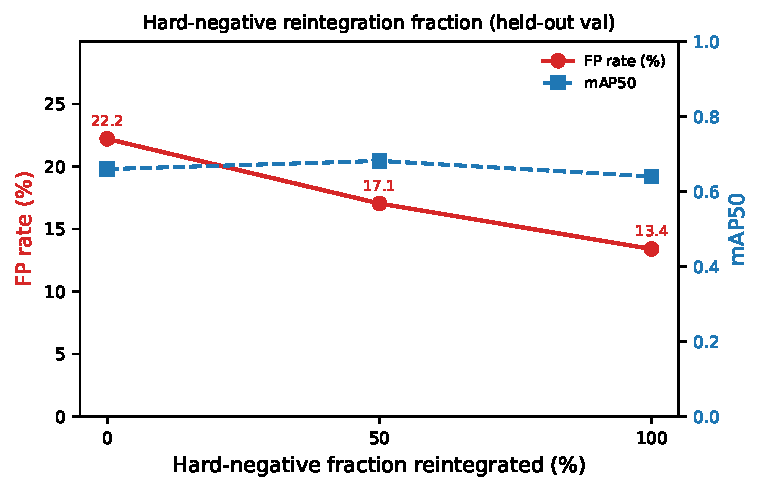
\includegraphics[width=\linewidth,height=0.3\textheight,keepaspectratio]{figures/ablation_hn.pdf}
\caption{Hard-negative reintegration fraction. At \(N=18\) the fraction barely
matters; the FN-rebalanced arm is what moves the false-positive rate.}
\label{fig:ablation_hn}
\end{figure}

\section{Data \& Code Availability}
The benchmark that produced every number in this paper lives in
\texttt{benchmark\_outlier\_analysis.py}, seeded at 42 and fully reproducible
on CPU; the raw evidence is committed under \texttt{evidencias/}. To
reproduce the production pipeline that hosts step 13, clone the
\texttt{wyoloservice2\_production} repository and run
\texttt{docker-compose up -d}. This work is released under a Dual Licensing
Model: PolyForm Noncommercial for research use and AGPLv3 for open-source use.

\section{Broader Impact}
The carbon argument is direct: targeted data corrections replace full
retraining cycles. Every epoch a worker does not run on an edge node is energy
it does not burn~\cite{zhou2019edge}. The safety argument is shift-left: a
model that surfaces its own failures during validation fails earlier and
cheaper than one that fails in production. The dual-use concern is real but
contained: the module optimizes detectors, and the same capability can improve
surveillance systems. We believe the efficiency and transparency gains
outweigh that risk, and we document the protocol precisely so the community
can audit it.

\section{Conclusion \& Future Work}
We presented the OutlierFailureAnalyzer, evaluated it without data leakage on
COCO128, and established a counter-intuitive result: hard-negative crops alone
improve false-positive rates at small \(N\), cutting the high-confidence rate
from 8.33\% to 2.00\%, while naive false-negative rebalancing backfires,
raising false positives without recovering recall. Two lines of future work
follow. Larger \(N\) on real industrial data would confirm the effect size.
And the module could be extended to schedule when to trigger a
retrain---measuring failure drift before committing the compute.

\section*{Acknowledgments}
This work was supported by the wisrovi-suit project and the open tooling
ecosystem it maintains.

\bibliographystyle{IEEEtran}
\bibliography{references}

\end{document}